% class used: https://www.maths.ox.ac.uk/members/it/faqs/latex/thesis-class
% also used https://github.com/brendanfong/dphil for inspiration

\documentclass[12pt]{ociamthesis}  % default square logo
%\documentclass[12pt,beltcrest]{ociamthesis} % use old belt crest logo
%\documentclass[12pt,shieldcrest]{ociamthesis} % use older shield crest logo

%load any additional packages
\usepackage{amssymb}
% \usepackage{amsmath}
\usepackage{mathtools} % includes amsmath
% \allowdisplaybreaks[4]
\allowdisplaybreaks
\usepackage{subcaption}
\usepackage{graphicx}
\usepackage{tikzit}
\usepackage{xcolor}
\usepackage{listings}
\usepackage{xparse}
\usepackage{kantlipsum}
\usepackage{algorithm}
\usepackage{algorithmicx}
\usepackage[noend]{algpseudocode}
\usepackage{tikz}
\usetikzlibrary{arrows.meta, chains, positioning, shapes.geometric, decorations.pathreplacing}
\usepackage{siunitx}
\usepackage{booktabs}
\usepackage{multirow}
\usepackage[stable]{footmisc}

\tikzset{FlowChart/.style={
    startstop/.style = {rectangle, draw, fill=red!30, minimum width=3cm, minimum height=1cm,
      on chain, join=by arrow},
    process/.style = {rectangle, rounded corners, draw, fill=blue!30, text width=5cm,
      minimum height=1cm, align=center, on chain, join=by arrow},
    decision/.style = {diamond, aspect=1.3, draw, fill=green!30, minimum width=3cm,
      minimum height=1cm, align=center, on chain, join=by arrow},
    arrow/.style = {thick,-Triangle}
  }
}

\input{zx.tikzstyles}
\input{zx.tikzdefs}

\newcommand{\bra}[1]{\ensuremath{\left\langle #1 \right|}}
\newcommand{\ket}[1]{\ensuremath{\left|  #1 \right\rangle}}
\newcommand{\braket}[2]{\ensuremath{\langle#1|#2\rangle}}
\newcommand{\ketbra}[2]{\ensuremath{\ket{#1}\!\bra{#2}}}

% commands for pseudocode
\newcommand*\Let[2]{\State #1 $\gets$ #2}
\algrenewcommand\algorithmicrequire{\textbf{Precondition:}}
\algrenewcommand\algorithmicensure{\textbf{Postcondition:}}

\NewDocumentCommand{\codeword}{v}{
  \texttt{\textcolor{gray}{#1}}
}
\lstset{language=C,keywordstyle={\bfseries \color{blue}}}


%input macros (i.e. write your own macros file called mymacros.tex
%and uncomment the next line)
%\include{mymacros}

\title{Vanishing 2-Qubit Gates with\\[1ex]     %your thesis title,
        Non-Simplification ZX-Rules}   %note \\[1ex] is a line break in the title

% \author{Ryan Krueger}            %your name
\author{Candidate Number: 1048427}
% \college{Christ Church College}  %your college
\college{Word Count: 7458}

%\renewcommand{\submittedtext}{change the default text here if needed}
\degree{Master of Science in Mathematical Sciences}     %the degree
\degreedate{Trinity 2021}         %the degree date

%end the preamble and start the document
\begin{document}

%this baselineskip gives sufficient line spacing for an examiner to easily
%markup the thesis with comments
\baselineskip=18pt plus1pt

%set the number of sectioning levels that get number and appear in the contents
\setcounter{secnumdepth}{3}
\setcounter{tocdepth}{3}


\maketitle                  % create a title page from the preamble info
% \begin{dedication}
Lorem ipsum dolor sit amet, consectetur adipiscing elit, sed do eiusmod tempor incididunt ut labore et dolore magna aliqua. Ut enim ad minim veniam, quis nostrud exercitation ullamco laboris nisi ut aliquip ex ea commodo consequat.
\end{dedication}
        % include a dedication.tex file
\begin{acknowledgements}
  I would like to thank my supervisor Aleks Kissinger for coordinating this project with me and for his mentorship throughout the year.
  I would also like to thank my family for their love and support.
\end{acknowledgements}
  % include an acknowledgements.tex file
\begin{abstract}
Lorem ipsum dolor sit amet, consectetur adipiscing elit, sed do eiusmod tempor incididunt ut labore et dolore magna aliqua. Ut enim ad minim veniam, quis nostrud exercitation ullamco laboris nisi ut aliquip ex ea commodo consequat.
\end{abstract}
          % include the abstract

\begin{romanpages}          % start roman page numbering
\tableofcontents            % generate and include a table of contents
% \listoffigures              % generate and include a list of figures
\end{romanpages}            % end roman page numbering

%now include the files of latex for each of the chapters etc
\chapter[Introduction]{Introduction} \label{ch:intro}

% https://quantumcomputing.stackexchange.com/questions/1885/what-is-meant-by-noisy-intermediate-scale-quantum-nisq-technology

Quantum computing arose from the idea that the ``bugs'' of quantum mechanics (e.g., superposition) may serve as useful features for information processing.
Since this framing was posed in the late 1970's, a rich theory of quantum information has developed that treats a \emph{qubit}, a superposition of two classical bits, as the basic unit of information.
Quantum information science is an exciting field of work as many quantum algorithms have been discovered that offer significant speedups from their classical counterparts (e.g., Shor's algorithm for integer factorization).
However, like the formulation of the Turing machine decades before the invention of the transistor, efforts to engineer a real-world quantum computer that can implement these theories are in their infancy.
% Indeed, reminiscent of early experimentation with vacuum tubes and relays for implementing classical logic, finding the optimal physical implementation of a qubit remains an active area of research.

The current state-of-the-art are so-called noisy intermediate-scale quantum (NISQ) computers~\cite{preskill2018quantum}.
These are devices without enough qubits to spare for error correction (i.e., noisy) and with a relatively small qubit number (i.e., intermediate-scale).
With \textasciitilde 50 qubits, NISQ devices cannot run particularly resource-intensive quantum algorithms (e.g., Shor's algorithm at a meaningful scale) but do afford the occasional speedup over classical computers.
To stress these capabilities, there is significant effort towards minimizing \emph{quantum circuits}, the standard model for a quantum computation, to mitigate noise and decoherence.
More formally, this field is known as \emph{quantum circuit optimization}.
\iffalse
% FIXME: noise and decoherence are problems
FIXME: Order of 50 qubits.
FIXME: ``Randomizing influences such as heat in the surroundings might nudge a qubit to switch, say, from a 1 to a 0 state, a phenomenon known as noise.''
FIXME: ``The quantum information that they hold can become scrambled within a fraction of a second, a problem called decoherence.''
FIXME: ``to solve a factoring problem that is not feasible for a classical computer, we will require millions of qubits. This overhead is required for error correction, since most algorithms we know are extremely sensitive to noise''
FIXME: ``Once this is done, we'll be in a strange era. We'll know that devices can do things that classical computers can't, but they won't be big enough to provide fault-tolerant implementations of the algorithms we know about. Preskill coined the term 'Noisy Intermediate-Scale Quantum' to describe this era. Noisy because we don't have enough qubits to spare for error correction, and so we'll need to directly use the imperfect qubits at the physical layer. And 'Intermediate-Scale' because of their small (but not too small) qubit number.''

FIXME: Crucial is testing and running things on them (As with early operating systems etc, NISQ machines warrant ... software?). To do so, quantum circuits have to be as SMALL as possible (to reduce noise) (because main challenge/bottleneck in NISQ is effects, etc, and these have to be minimized). This has spurred the field of quantum circuit optimization.
\fi


% The ZX-calculus is a graphical formalism, rooted in category theory, for representing quantum circuits as \emph{ZX-diagrams} and manipulating them via a set of rewrite rules.
% This language provides a unique setting for circuit optimization as ZX-diagrams provide a lower-level represention of quantum circuits that can be deformed arbitrarily.
The ZX-calculus, a graphical formalism for quantum circuits rooted in category theory, provides a unique setting for circuit optimization.
In this language, quantum circuits are represented as \emph{ZX-diagrams} that are manipulated via a set of rewrite rules.
ZX-diagrams provide a lower-level representation for quantum computations and can be deformed arbitrarily, enriching the space of possible simplifications.
While there is no known procedure for recovering a quantum circuit from a general ZX-diagram, subsets of transformations have been identified that preserve circuit extractability.
These transformations have enabled a suite of circuit optimization procedures in the ZX-calculus (e.g., for reducing T-count) with various tradeoffs.

Still, circuit extraction from a ZX-diagram remains a bottleneck for optimization;
the best known extraction procedures can introduce an unwieldy degree of complexity in the resulting circuit.
For example, circuit extraction can introduce many CNOT gates which are particularly problematic on NISQ devices.
Interestingly, however, closely related ZX-diagrams can induce drastically different circuits.
Current optimization procedures employing the ZX-calculus do not exploit this fact (e.g., by searching local variants) but rather return a ZX-diagram (or its associated circuit) once no more graph simplifications can be applied.

In this thesis, we explore the role that such a search over local variants of ZX-diagrams could play in circuit optimization.
More specifically, we apply various search procedures (i.e., simulated annealing and genetic algorithms) over the application of congruences (i.e., non-simplification rewrite rules) to a fully simplified ZX-diagram.
We use two congruences that arise from the graph-theoretic notions of local complementation and pivoting.
We find that our optimization strategy reliably outperforms off-the-shelf methods on randomly generated circuits with $<10$ qubits and on a set of benchmark circuits with $\leq 14$ qubits.
Most notably, on the benchmark circuits, our method eliminates up to 46\% of 2-qubit gates and consistently reduces the circuit complexity by an additional 15-30\%.
% rewrite rules that do not necessarily simplify the graph itself but may reduce the complexity of the associated circuit.
% By default, we apply this search over an already simplified diagram (via off-the-shelf methods) but also explore more general strategies for combining these search procedures and/or rewrite rules with existing optimization procedures.
% When seeding this search with a pre-simplified ZX-diagram (obtained via off-the-shelf methods), we find that FIXME. % we can reduce the 2-qubit-count by an average of FIXME \% without increasing the number of T-gates. (Note to RK: but single-qubit gate count is increased).
% We find that (FIXME: this combination is effective for reducing the 2-qubit count on random circuits when the number of qubits is less than 10).

\chapter[Background]{Background} \label{ch:bg}

% https://en.wikipedia.org/wiki/Quantum_computing
% https://en.wikipedia.org/wiki/Quantum_circuit
% https://en.wikipedia.org/wiki/Quantum_logic_gate

To understand quantum circuit optimization in the ZX-calculus, one first must understand quantum circuits and the ZX-calculus.
In this section we provide the requisite background in both of these, preceded by a brief discussion on qubits.
We conclude this section with an overview of quantum circuit optimization in the ZX-calculus.

\section{Qubits}\label{sec:qubits}

A classical bit has a value of 0 or 1.
A quantum bit, or \emph{qubit}, encodes a quantum superposition of these two values and therefore more information than a classical bit.
In the traditional bra-ket notation of quantum mechanics, a qubit is represented by a vector in $\mathbb{C}^2$,
\begin{align*}
  |\psi\rangle = \lambda_1 |0\rangle + \lambda_2 |1\rangle = \begin{pmatrix}\lambda_1 \\ \lambda_2 \end{pmatrix}
\end{align*}
where
\begin{align*}
  & |0\rangle = \begin{pmatrix}1 \\ 0\end{pmatrix} \\
  & |1\rangle = \begin{pmatrix}0 \\ 1\end{pmatrix}
\end{align*}
and $\lambda_1$ and $\lambda_2$ are the probability amplitudes of observing $|0\rangle$ and $|1\rangle$ upon measurement in this basis, respectively.
Notably, qubits can be written with respect to any orthonormal basis.
The set $\{|0\rangle, |1\rangle\}$ is known as the \emph{computational} basis.
Another common basis is the +/- basis, where
\begin{align*}
  & |+\rangle = \frac{|0\rangle + |1\rangle}{\sqrt{2}} \\
  & |-\rangle = \frac{|0\rangle - |1\rangle}{\sqrt{2}}
\end{align*}
The computational and +/- bases are also known as the Z and X bases, respectively.

More generally, a system of $n$ qubits is represented by the tensor product of the individual states.
So, an $n$-qubit state corresponds to a $2^{n}$-dimensional vector.
For example, the two-qubit state with both qubits in $|0\rangle$ is
\begin{align*}
  |0\rangle \otimes |0\rangle = |00\rangle = \begin{pmatrix}1 \\ 0 \\ 0 \\ 0\end{pmatrix}
\end{align*}
In the ZX-calculus and this work, qubits are abstracted as wires in string diagrams.
However, this definition is included both for completeness and to aid understanding of quantum circuits.

\begin{figure}
\centering
\begin{subfigure}{.5\textwidth}
  \centering
  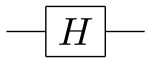
\includegraphics[width=.4\linewidth]{img/had}
  \caption{The Hadamard gate.}
  \label{fig:had}
\end{subfigure}%
\begin{subfigure}{.5\textwidth}
  \centering
  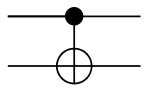
\includegraphics[width=.4\linewidth]{img/cnot}
  \caption{The CNOT gate. The top and bottom qubits are the control and target, respectively.}
  \label{fig:cnot}
\end{subfigure}
\caption{
  The circuit representation of two common quantum logic gates.
  Wires represent qubits and boxes represent quantum logic gates.
  Quantum circuits are read from left to right.
}
\label{fig:test}
\end{figure}


\section{Quantum Circuits}\label{sec:qcircs}

A quantum circuit models a quantum computation as a sequence of discrete gates.
In the traditional notation with qubits as vectors in $\mathbb{C}^2$, quantum gates correspond to unitary matrices.
For example, the Hadamard gate, a quantum gate that acts on a single qubit and maps
\begin{align*}
  & |0\rangle \mapsto \frac{|0\rangle + |1\rangle}{\sqrt{2}} \\
  & |1\rangle \mapsto \frac{|0\rangle - |1\rangle}{\sqrt{2}}
\end{align*}
has the matrix form
\begin{align*}
  H = \frac{1}{\sqrt{2}}\begin{bmatrix}1 & 1 \\ 1 & -1\end{bmatrix}
\end{align*}
Figure \ref{fig:had} depicts the circuit representation of the Hadamard gate.
Note that $|+\rangle = H|0\rangle$ and $|-\rangle = H|1\rangle$.
An important family of single-qubit gates are the \emph{phase shift} gates that modify the phase of the quantum state by some $\alpha$.
A phase shift gate maps
\begin{align*}
  & |0\rangle \mapsto |0\rangle \\
  & |1\rangle \mapsto e^{i\alpha}|1\rangle \\
\end{align*}
and has the matrix form
\begin{align*}
  R_{\alpha} = \begin{bmatrix}1 & 0 \\ 0 & e^{i\alpha}\end{bmatrix}
\end{align*}
Examples of phase gates are the T-gate ($\alpha = \frac{\pi}{4}$) and the S-gate ($\alpha = \frac{\pi}{2}$).
Phase gates where $\alpha$ is a multiple of $\pi / 2$ are called \emph{Clifford} gates.

Quantum gates are not restricted to acting on single qubits.
For example, the controlled-NOT (CNOT) gate acts on two qubits and flips the second (target) qubit only when the first (control) qubit is $|1\rangle$.
The CNOT gate is typically depicted as shown in Figure \ref{fig:cnot} and has the following matrix form:
\begin{align*}
  CNOT = \begin{bmatrix}1 & 0 & 0 & 0 \\0 & 1 & 0 & 0 \\ 0 & 0 & 0 & 1\\0 & 0 & 1 & 0\end{bmatrix}
\end{align*}
In general, an $n$-qubit gate is represented by a $2^n$-dimensional unitary.
However, attention is typically restricted to single- and 2-qubit gates as it is well known that the Clifford + T gate set, consisting of the H, T, S, and CNOT gates, is \emph{universal} -- any other operation can be represented by a finite sequence from this set.
The \emph{Clifford circuits} are those that can be generated by $\{H, S, CNOT\}$.
As the T and S gates are instances of phase shift gates, $\{H, R_{\alpha}, CNOT\}$ is also universal though in practice any non-Clifford phase gate is implemented with T gates. % FIXME: Is this true?
% A subset of all operators, \emph{Clifford circuits} are those that can be generated by $\{H, S, CNOT\}$ (i.e., by fixing $\alpha = \pi / 2$).

Quantum gates can be composed sequentially or in parallel.
Consider two gates $A$ and $B$.
The effect of $B$ applied in series after $A$ can be described by a single gate (i.e., linear map) via matrix multiplication (i.e., $B \cdot A$).
Alternatively, the tensor product is used to describe A and B in parallel (i.e., $B \otimes A$).
For example, the simple circuit shown in Figure \ref{fig:simple-trad} can be described by the following linear map:
\begin{align*}
  (\mathbb{I} \otimes CNOT) \cdot (\mathbb{I} \otimes H \otimes \mathbb{I}) \cdot (CNOT \otimes \mathbb{I}) \cdot (S \otimes \mathbb{I} \otimes \mathbb{I})
\end{align*}



\begin{figure}
\centering
\tikzfig{ZX-rules}
\caption{
  The rules of the ZX-calculus.
  All rules hold with the colors interchanged and for $\alpha, \beta \in [0, 2 \pi)$.}
\label{fig:zx-rules}
\end{figure}



\section{ZX-Calculus}\label{sec:zx}

The ZX-calculus is a graphical language for representing and reasoning about quantum processes.
Quantum processes are represented by \emph{ZX-diagrams} which consist of \emph{wires} and \emph{spiders}.
Spiders can have an arbitrary number of inputs and outputs and come in two flavors: Z spiders (shown in green) and X spiders (shown in red).
As with quantum circuits, a ZX-diagram is interpreted from left to right.

ZX-diagrams abstract away the complexities of linear algebra and tensor products from traditional formalisms of quantum processes.
Wires still represent qubits while spiders provide a general form for linear maps, where
\begin{align*}
  & \tikzfig{Zsp-a} := \ketbra{0...0}{0...0} + e^{i\alpha}\ketbra{1...1}{1...1} \\
  & \tikzfig{Xsp-a} := \ketbra{+...+}{+...+} + e^{i\alpha}\ketbra{-...-}{-...-}
\end{align*}
Two diagrams can be composed in serial by joining the outputs of the first to the inputs of the second, or in parallel by stacking the two diagrams.

From this definition, we can identify the diagrammatic represenations for several common components of quantum computation:
\[
\begin{array}{rclcrcl}
\tikzfig{ket-+} & = & \ket{0} + \ket{1} \ \propto \ket{+} &
\qquad\qquad &
\tikzfig{ket-0} & = & \ket{+} + \ket{-} \ \propto \ket{0} \\
&\quad& & & \quad \\
\tikzfig{Z} & = & \ketbra{0}{0} - \ketbra{1}{1} = Z &
&
\tikzfig{X} & = & \ketbra{+}{+} - \ketbra{-}{-} = X
\end{array}
\]
where $Z$ and $X$ are the corresponding Pauli matrices.
Note that spiders without any inputs can be regarded as qubit state preparations.
The Hadamard gate is so pervasive that it merits shorthand notation;
we use a yellow square to represent the Hadamard gate as shown below
% \ctikzfig{had-alt}
\begin{equation}\label{eq:had-short}
  \tikzfig{had-alt}
\end{equation}
and replace a Hadamard gate between two spiders with a blue dashed edge:
\ctikzfig{blue-edge-def}

We can also reason about ZX-diagrams.
The first rule for determining equality is that \emph{only connectivity matters} (OCM).
In other words, two ZX-diagrams are equal when one can be deformed into the other (e.g., via moving vertices around in the plane or bending wires) while maintaining connectivity and the order of the inputs and outputs.
In addition to this OCM principle, the ZX-calculus includes a primary set of rewrite rules as shown in Figure \ref{fig:zx-rules}.
These rules only hold up to non-zero scalar factors, though these scalars are typically ignored as they correspond to negligible differences in global phase.
Additional rules can be derived from this set, such as the antipode rule
\ctikzfig{hopf-rule}
and the $\pi$-copy rule
\ctikzfig{picopy-rule}

All quantum circuits can be translated to ZX-diagrams.
This is a consequence of the fact that the following universal gate set can be easily represented in the ZX-calculus:
\begin{align*}
CNOT & = \tikzfig{cnot} &
R_{\alpha} & = \tikzfig{Z-a} &
H & = \tikzfig{h-alone}
\end{align*}
In the CNOT diagram, the green and red spiders are the control and target qubits, respectively.
As an example, Figure \ref{fig:simple-circ} depicts both the traditional and diagrammatic representations of a simple quantum circuit.



\begin{figure}
\centering
\begin{subfigure}[t]{.3\textwidth}
  \centering
  % 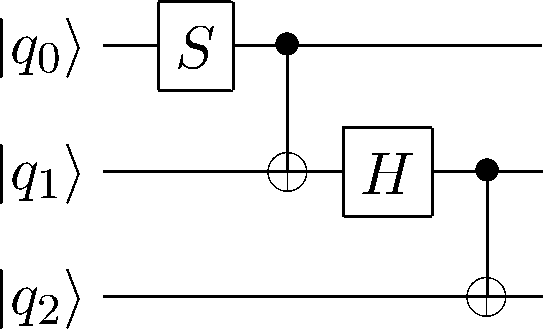
\includegraphics[width=.4\linewidth]{img/traditional.png}
  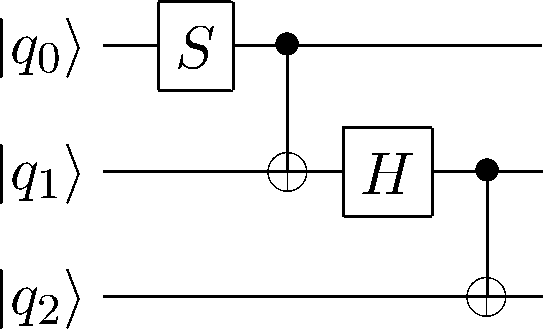
\includegraphics[width=4cm]{img/traditional.png}
  \caption{Traditional notation}
  \label{fig:simple-trad}
\end{subfigure}%
\begin{subfigure}[t]{.7\textwidth}
  \centering
  \resizebox{9cm}{!}{\begin{tikzpicture}
	\begin{pgfonlayer}{nodelayer}
		\node [style=none] (0) at (-5.75, 1) {};
		\node [style=none] (1) at (-5.75, 0) {};
		\node [style=none] (2) at (-5.75, -1) {};
		\node [style=Z phase dot] (3) at (-4.75, 1) {$\frac{\pi}{2}$};
		\node [style=X dot] (4) at (-3.75, 0) {};
		\node [style=Z dot] (5) at (-3.75, 1) {};
		\node [style=Z dot] (6) at (-2.75, 0) {};
		\node [style=X dot] (7) at (-1.75, -1) {};
		\node [style=Z dot] (8) at (-1.75, 0) {};
		\node [style=none] (9) at (-0.75, 1) {};
		\node [style=none] (10) at (-0.75, 0) {};
		\node [style=none] (11) at (-0.75, -1) {};
		\node [style=none] (12) at (0.75, 1) {};
		\node [style=none] (13) at (0.75, 0) {};
		\node [style=none] (14) at (0.75, -1) {};
		\node [style=Z phase dot] (15) at (1.75, 1) {$\frac{\pi}{2}$};
		\node [style=X dot] (16) at (1.75, 0) {};
		\node [style=Z dot] (17) at (2.75, 0) {};
		\node [style=X dot] (18) at (2.75, -1) {};
		\node [style=none] (19) at (3.75, 1) {};
		\node [style=none] (20) at (3.75, 0) {};
		\node [style=none] (21) at (3.75, -1) {};
		\node [style=none] (22) at (0, 0) {=};
	\end{pgfonlayer}
	\begin{pgfonlayer}{edgelayer}
		\draw (0.center) to (3);
		\draw (1.center) to (4);
		\draw (2.center) to (7);
		\draw (3) to (5);
		\draw (4) to (5);
		\draw [style=hadamard edge] (4) to (6);
		\draw (5) to (9.center);
		\draw (6) to (8);
		\draw (7) to (8);
		\draw (7) to (11.center);
		\draw (8) to (10.center);
		\draw (12.center) to (15);
		\draw (13.center) to (16);
		\draw (14.center) to (18);
		\draw (15) to (16);
		\draw (15) to (19.center);
		\draw [style=hadamard edge] (16) to (17);
		\draw (17) to (18);
		\draw (17) to (20.center);
		\draw (18) to (21.center);
	\end{pgfonlayer}
\end{tikzpicture}
}
  \caption{ZX-diagram}
  \label{fig:simple-zx}
\end{subfigure}
\caption{A simple 3-qubit quantum circuit shown in both the traditional notation and as a ZX-diagram.}
\label{fig:simple-circ}
\end{figure}


\section{Circuit Optimization in the ZX-Calculus}\label{sec:zx-circ-opt}

% Note: be careful about circuit-like graph. This is stricter than circuit-extractability (from_graph vs. extract_circuit

The goal of quantum circuit optimization is to simplify quantum circuits (e.g., via reducing the number of gates) to reduce noise and decoherence when run on modern quantum computers.
More specifically, the T-count and 2-qubit-count are typically targeted; fault tolerant implementations of T gates generally require an order of magnitude more resources than Clifford gates~\cite{campbell2017roads}, and the fidelity of single-qubit gates is demonstrably higher than that of 2-qubit gates~\cite{ballance2016high}.
It is standard to perform optimizations at the circuit-level.
Examples of circuit-level optimizations are 3-qubit gate decomposition and cancelling back-to-back CNOT gates.

The ZX-calculus enables circuit optimization at the graph-level, a more flexible setting that is well-studied in its own right.
Such an optimization involves converting a circuit to a ZX-diagram, simplifying the diagram, and converting the diagram back to a circuit. % TODO: Could have a figure for this pipeline
However, there is no known general-purpose procedure for recovering a quantum circuit from a generic ZX-diagram.
This restricts the space of permissible simplifications to those that preserve whichever diagrammatic properties are required by the extraction procedure.


\begin{figure}
\centering
\tikzfig{graph-like-ex}
\caption{An example of a ZX-diagram and an equivalent, graph-like ZX-diagram.}
\label{fig:graph-like}
\end{figure}

In 2020, Duncan et al. reported an extraction procedure that enabled current best practices~\cite{duncan2020graph}.
Firstly, this procedure operates on \emph{graph-like} ZX-diagrams.
A ZX-diagram is graph-like when:
\begin{enumerate}
\item
  All spiders are Z-spiders.
\item
  Z-spiders are only connected via Hadamard edges
\item
  There are no parallel Hadamard edges or self-loops
\item
  Every input or output is connected to a Z-spider and every Z-spider is connected to at most one input or output
\end{enumerate}
Every ZX-diagram is equal to a graph-like diagram (see Figure \ref{fig:graph-like} for an example), and this form admits an underlying graph structure that permits graph-theoretic analyses.
Secondly, this procedure requires that the underlying graph of the input ZX-diagram satisfies a graph-theoretic invariant called \emph{focused generalized flow} (focused gFlow). % which guarantees that FIXME.
Given such an input ZX-diagram, extraction proceeds in such a way that each non-zero phase corresponds to one phase gate in the resulting circuit but each edge can correspond to multiple CNOTs.
For this reason, local changes in a ZX-diagram (e.g., connectivity) can have significant effects on the complexity of the associated circuit.
Importantly, this extraction procedure is not optimal;
if a given circuit is converted to a ZX-diagram and the extraction procedure is immediately applied, the extracted circuit is often more complex than the original circuit.
In particular, this procedure can drastically increase the number of 2-qubit gates.
For more details on the extraction procedure or focused gFlow, see \cite{duncan2020graph}.

% Note: be careful. focused gFlow is something that exists. E.g., "The existence of a focused gFlow is preserved by local complementation and pivoting"

Alongside this extraction procedure, Duncan et al. also introduced an optimization procedure that relies on focused gFlow-preserving graph simplifications.
More specifically, this procedure relies on two graph-theoretic transformations that each correspond to rewrite rule in the ZX-calculus: \emph{local complementation} and \emph{pivoting}.
Given a graph $G$ and some vertex $u$ of $G$, the \emph{local complementation} of $G$ according to $u$, denoted $G \star u$, is the graph in which the connectivity of all pairs of neighbors of $u$ is inverted.
For example,
\begin{equation*}
G\quad\tikzfig{graph1-lab}\qquad\qquad G\star a\quad\tikzfig{graph1-lab-1}
\end{equation*}
Given a ZX-diagram, local complementation can be induced in the underlying graph structure while maintaining equality by applying an $X_{-\pi/2}$ gate on (the spider corresponding to) $u$ and a $Z_{\pi/2}$ gate to its neighbors~\cite{duncan2009graph}:
% \ctikzfig{local-comp-ex}
\begin{equation}\label{eq:gs-local-comp}
  \tikzfig{local-comp-ex}
\end{equation}
Relatedly, given two connected vertices $u$ and $v$ in $G$, the \emph{pivot} of $G$ along the edge $uv$ is the graph $G \wedge uv :=G \star u \star v \star u$.
In practice, this consists of complementing the edges between three subsets of vertices: (1) the common neighborhood of $u$ and $v$, (2) the exclusive neighborhood of $u$, and (3) the exclusive neighborhood of $v$:
\[G \quad\tikzfig{pivot-L}\qquad\qquad \quad G\wedge uv \quad\tikzfig{pivot-R}
\]
Again, given a ZX-diagram, the rewrite rule reported in \cite{duncan2013pivoting} introduces a pivot by applying Hadamard gates on $u$ and $v$ and $Z_{\pi}$ gates on their common neighborhood:
% \ctikzfig{pivot-desc}
\begin{equation}\label{eq:gs-pivot}
  \tikzfig{pivot-desc}
\end{equation}
Each rewrite rule can be extended to a simplification by performing local complementation (resp. pivoting), removing the vertex (resp. the pair of vertices), and updating the phases:
\ctikzfig{lc-simp}
\ctikzfig{pivot-simp}
Importantly, the existence of a focused gFlow is preserved in both cases.
At a high-level, optimization can then be performed by applying these simplifications to fixpoint and extracting a circuit from the resulting ZX-diagram.
Details on this optimization procedure and proofs of the simplification rules or their focused gFlow-preservation can be found in \cite{duncan2020graph}.
A variant of this procedure is implemented in the \codeword{full_reduce} method of the PyZX library.

One issue with \codeword{full_reduce} is its reliance on circuit extraction; it is not uncommon that the circuit extracted from the final, simplified ZX-diagram has more gates than the input circuit.
Kissinger and van de Wetering introduced an alternative optimization method that uses \emph{phase teleportation} to sidestep the issue of circuit extraction altogether~\cite{kissinger2019reducing}.
Crucially, simplification of the ZX-diagram is performed symbollically.
% In addition to the aforementioned rules, this procedure uses several new rewrite rules that remove interior Pauli spiders at the cost of introducing \emph{phase-gadgets}, a ZX-diagrammatic motif.
This symbolic simplification leverages the fact that several rewrite rules involving \emph{phase-gadgets}, a particular ZX-diagrammatic motif, correspond to changes in the original phases.
Therefore, non-Clifford phases can potentially cancel or combine with each other while leaving the original graphical structure of the ZX-diagram intact.
% By exploiting a particular motif, the \emph{phase-gadget}, particular rewrite rules correspond to changes in the phases of the original ZX-diagram.
% So, as simplification proceeds using both the aforementioned rules as well as several new rewrite rules (that remove interior Pauli spiders at the cost of introducing phase-gadgets), changes in the original diagram are simply tabulated, absolving the need for extraction.
So, as simplification proceeds, application of these rules is simply tabulated to enable reconstruction of a final circuit with the same connectivity but a possible reduction in non-Clifford gates (and therefore T-count).
% using both the rules described above as well as several new rewrite rules that remove any remaining interior Pauli spiders at the cost of introducing \emph{phase-gadgets}, a particular ZX-diagrammatic motif.
% Instead, the ZX-diagram is first simplified using both rules described above as well as several new rewrite rules that remove any remaining interior Pauli spiders at the cost of introducing \emph{phase-gadgets}, a particular ZX-diagrammatic motif.
Importantly, using phase teleportation rather than circuit extraction ensures that the number of 2-qubit and Hadamard gates is unchanged. % while the T-count can be reduced.
By changing the angles of many non-Clifford phase gates to either 0 or multiples of $\pi /2$, this procedure can also make a circuit-level optimization procedure much more effective.
% In this way, this simplification procedure never increases the number of 2-qubit or Hadamard gates and can only reduce T-count.
This procedure is implemented in the \codeword{teleport_reduce} method of PyZX.
% and gates are always paplied between the same pairs of qubits as before
% non-Clifford phases can potentially cancel or combine with each other

\chapter[Methods]{Methods} \label{ch:methods}

At a high level, the goal of any quantum circuit optimization is to reduce the complexity of the input circuit.
A core assumption of circuit optimization in the ZX-calculus is that ZX-diagrams with fewer spiders typically correspond to simpler circuits.
Earlier, however, we noted that local changes (e.g., connectivity) in a ZX-diagram can drastically affect the complexity of the associated circuit obtained via extraction.
However, no existing optimization procedure over ZX-diagrams addresses this and searches this local space.
The \codeword{full_reduce} method described in Section \ref{sec:zx-circ-opt} is the quintessential example of this lost opportunity.
After the two simplification rules can no longer be applied, the final circuit is taken to be that which is extracted from the resulting simplified ZX-diagram;
however, there may be an equivalent ZX-diagram lurking nearby whose associated circuit is markedly less complex.

In this thesis, we explore the utility of searching this local space of equivalent ZX-diagrams.
To do so, we first need rewrite rules that modify a ZX-diagram in a manner other than spider removal that may reduce circuit complexity.
Indeed, a rule that introduces several additional spiders alongside changes in connectivity may in turn yield a less complex circuit.
We refer to these rewrite rules as \emph{congruences}.
Given a set of congruences, we then need a procedure to search the space of equivalent ZX-diagrams generated by an input ZX-diagram and these rules.
We can then devise strategies for incorporating this local search into existing methods for circuit optimization in the ZX-calculus.

We present the methods of our work in this order.
First, we generalize the original (non-simplification) variants of local complementation and pivoting to ZX-diagrams with arbitrary phases.
We then describe two search procedures, simulated annealing (SA) and genetic algorithms (GA).
% for searching the space of ZX-diagrams generated by these congruences.
We also define a measure of circuit complexity and discuss candidate objective functions to guide search. % to the ZX-diagram whose circuit has minimal complexity.
Lastly, we discuss how this search can be incorporated into existing optimization pipelines.
% Our primary strategy is to first simplify a ZX-diagram using existing methods and subsequently search the local variants of the simplified ZX-diagram.
% Alternatively, we can use SA or GA as the principal means of optimization.
% In this more ambitious approach, congruences can be combined with simplification rules to form an action set over which search is applied.

\section{Congruences}\label{sec:congruences}

The non-simplification versions of local complementation and pivoting presented in Section \ref{sec:zx-circ-opt} embody the desired properties of congruences.
They change the connectivity of the ZX-diagram without introducing an unwieldy number of additional gates, presenting an opportunity for a potential reduction in circuit complexity.
However, Equations \ref{eq:gs-local-comp} and \ref{eq:gs-pivot} only apply to spiders with zero phase and a single wire.

% Useful for spacing:
% https://tex.stackexchange.com/questions/54587/vertical-spacing-within-align-environment-accounting-for-fractions
We can apply the rules of the ZX-calculus and Equation \ref{eq:gs-local-comp} to generalize local complementation to arbitrary phases ($\alpha_i, \beta_i \in [0, 2 \pi)$):
% note: can do \tag{\theequation} to get a number
% {\allowdisplaybreaks
\begin{spreadlines}{0.8em}% tweak
  \begin{align*}
    \tikzfig{gen-lc-single/0} &\stackrel{(\bm f)}{=} \tikzfig{gen-lc-single/1} \\
    &\stackrel{(\ref{eq:gs-local-comp})}{=} \tikzfig{gen-lc-single/2} \\
    &\stackrel{(\bm i1)}{=} \tikzfig{gen-lc-single/3} \\
    &\stackrel{(\bm f)}{=} \tikzfig{gen-lc-single/4} \\
    &\stackrel{(\bm f)}{=} \tikzfig{gen-lc-single/5} \\[0.8em]
    &\stackrel{(\ref{eq:had-short})}{=} \tikzfig{gen-lc-single/6}\stepcounter{equation}\tag{\theequation}\label{eq:gen-phase-lc}
  \end{align*}
\end{spreadlines}
% }
Equation \ref{eq:gen-phase-lc} can be easily extended to apply for an arbitrary number of wires connected to each spider:
% {\allowdisplaybreaks
\begin{spreadlines}{0.8em}% tweak
  \begin{align*}
    \tikzfig{gen-lc-mul/0} &\stackrel{(\bm f)}{=} \tikzfig{gen-lc-mul/1} \\
    &\stackrel{(\ref{eq:gen-phase-lc})}{=} \tikzfig{gen-lc-mul/2} \\
    &\stackrel{(\bm f)}{=} \tikzfig{gen-lc-mul/3}\stepcounter{equation}\tag{C1}\label{eq:gen-io-lc}
  \end{align*}
\end{spreadlines}
% }
% Equation \ref{eq:gs-pivot}:
Similarly, we can generalize pivoting to arbitrary phases:
% {\allowdisplaybreaks
\begin{spreadlines}{0.8em}% tweak
  \begin{align*}
    \tikzfig{gen-pivot-single/0} &\stackrel{(\bm f)}{=} \tikzfig{gen-pivot-single/1} \\
    &\stackrel{(\ref{eq:gs-pivot})}{=} \tikzfig{gen-pivot-single/2} \\
    &\stackrel{(\bm f)}{=} \tikzfig{gen-pivot-single/3}\stepcounter{equation}\tag{\theequation}\label{eq:gen-phase-pivot}
  \end{align*}
\end{spreadlines}
% }
Again, we can extend this rewrite rule for arbitrary wiring:
\begin{spreadlines}{0.8em}% tweak
  \begin{align*}
    \tikzfig{gen-pivot-mul/0} &\stackrel{(\bm f)}{=} \tikzfig{gen-pivot-mul/1} \\
    &\stackrel{(\ref{eq:gen-phase-pivot})}{=} \tikzfig{gen-pivot-mul/2} \\
    &\stackrel{(\bm f)}{=} \tikzfig{gen-pivot-mul/3}\stepcounter{equation}\tag{C2}\label{eq:gen-io-pivot}
  \end{align*}
\end{spreadlines}
% Equations \ref{eq:gen-io-lc} and \ref{eq:gen-io-pivot} will serve as our primary congruences -- those rewrite rules that, when applied, maintain a similar graph complexity but potentially reduce the circuit complexity.
Equations \ref{eq:gen-io-lc} and \ref{eq:gen-io-pivot} will serve as our primary congruences because they maintain a similar graph complexity (e.g., number of spiders and wires) but, due to their effects on connectivity, can produce circuits of varying complexities.
Equation \ref{eq:gen-io-lc} can be applied to any spider with a degree of more than 1.
Equation \ref{eq:gen-io-pivot} can be applied to any pair of connected spiders.


\section{Search Procedures}

The space of ZX-diagrams generated by an input ZX-diagram and these congruences is combinatorial and therefore cannot be searched exhaustively.
We can instead formulate this search as an optimization problem where the set of isomorphic ZX-diagrams are the states (reachable by congruence applications) that are evaluated by some quantitative measure of circuit complexity.
Here we describe two search procedures as well as several candidate objective functions that either measure circuit complexity directly or use ZX-diagrammatic properties as a proxy.

\subsection{Simulated Annealing}\label{sec:sa}

Simulated annealing is an optimization technique named after the annealing process in metallurgy in which a molten hot metal is cooled in a slow, controlled fashion in order for it to reach its most stable form.
In SA, this notion of slow cooling is interpreted as a slow decrease in the probability of accepting worse solutions.
In this way, the algorithm initially explores a broad region of the the search space and progressively narrows its scope.

More formally, the SA algorithm maintains a current state $s$ and at each step randomly considers some neighboring state $s^*$.
The algorithm then chooses whether or not to replace $s$ with $s^*$ via a Bernoulli random variable parameterized by the \emph{acceptance probability}, denoted $P(s, s^*, T)$. % FIXME: wrong subject for "denoted"?
The acceptance probability depends on (1) the \emph{energy} (i.e., objective) \emph{function}, and (2) the \emph{temperature}.
The energy function $E(s)$ assigns a score to each state (lower is better).
If $E(s') < E(s)$, then $s$ is always replaced with $s^*$ (i.e., $P(s, s^*, T) = 1$).
Otherwise, $P(s, s^*, T) = exp(-\frac{E(s^*) - E(s)}{T})$ where the temperature $T$ controls the likelihood of moving to a higher energy state.
Note that $P(s, s^*, T)$ is inversely proportional to $E(s^*) - E(s)$ and directly proportional to $T$.
Informally, this means that $s^*$ is more likely to be accepted if it is closer in energy to $s$ and with a higher temperature.
$T$ is initialized to some positive value and progressively decreases to zero.
At each step, $T$ is updated as $T = T * c$ where $c \in [0, 1)$ is the \emph{cooling} parameter. % FIXME: Change in code to always cool, not just when a change is made.
In this way, SA converges towards a greedy algorithm and is more likely to accept $s^*$ when $E(s^*) > E(s)$ early in search when $T$ is high.
The algorithm terminates when a maximum number of steps $k_{max}$ is reached (default: $k_{max} = 1000$).
Algorithm \ref{alg:sa} provides an overview of this procedure.

\begin{algorithm}[t]
  \caption{Simulated annealing
    \label{alg:sa}}
  \begin{algorithmic}[1]
    % \Require{$x$ and $y$ are packed \DNA{} strings of equal length $n$}
    % \Statex
    \Function{SimAnneal}{$s_0, T, c, k_{max}$}
      % \Let{$z$}{$x \oplus y$} \Comment{$\oplus$: bitwise exclusive-or}
      \Let{$s$}{$s_0$}
      \For{$i \gets 0 \textrm{ to } k_{max}$}
        \Let{$s^*$}{randomly sampled neighbor of $s$}
        \If{$E(s^*) < E(s)$ {\bf or} $\text{random}(0, 1) < exp(-\frac{E(s^*) - E(s)}{T})$}
          \Let{$s$}{$s^*$}
        \EndIf
        \Let{$T$}{$T * c$}
      \EndFor
      \State \Return{$s$}
    \EndFunction
  \end{algorithmic}
\end{algorithm}

In this work, the state is a ZX-diagram and neighbors are sampled via the probabilistic application of rewrite rules.
For example, to anneal using the rewrite rules described in Section \ref{sec:congruences}, $s^*$ would be sampled by first choosing one of Equation \ref{eq:gen-io-lc} or Equation \ref{eq:gen-io-pivot} and then choosing a spider or pair of connected spiders to which the rule will be applied.
Note that we use Equations \ref{eq:gen-io-lc} and \ref{eq:gen-io-pivot} by default but in theory any set of rewrite rules can be used.

\subsection{Genetic Algorithms}

Genetic algorithms are a class of optimization procedures inspired by the process of natural selection.
Rather than maintaining a single state (e.g., as in SA), a \emph{population} of candidate solutions is \emph{evolved}.
This evolution is guided by a \emph{fitness function} and operates via biologically inspired notions of \emph{mutation}, \emph{crossover}, and \emph{selection}.
In this work, we define fitness such that lower fitness is better to remain consistent with the energy function described in Section \ref{sec:sa}.
% For details on objective functions used to guide circuit optimization, see Section \ref{sec:obj-funcs}.

A genetic algorithm operates in the following general fashion.
First, a population of candidate solutions (i.e., \emph{mutants}) is randomly generated.
The population size is typically fixed to some $n_{mutants}$.
This initial population then evolves in a series of \emph{generations}.
Each generation consists of two parts: (1) selection and (2) application of genetic operators (e.g., mutation and crossover).
In the selection step, a score is assigned to each mutant via the fitness function and a new population is chosen given these scores.
For example, a naive selection method would set the population to $n_{mutants}$ copies of the best-scoring mutant.
Given this surviving population, the second step involves applying genetic operators to obtain a revised, diverse population.
The two most common genetic operators are mutation and crossover.
Analogous to mistakes being made during replication of a DNA sequence, a mutation operator involves randomly tweaking a single mutant.
In the case where mutants are represented as bit strings, the canonical example of a mutation operator is a bit-flip.
Alternatively, a crossover operator produces a new mutant given two or more existing mutants;
this is analogous to reproduction and biological crossover.
For example, given two mutants represented as strings, a new mutant can be generated by swapping the two segments defined by a random position.
Evolution proceeds for $n_{gens}$ generations and the algorithm returns the mutant with the highest fitness throughout search.
This process is summarized in Figure \ref{fig:ga}.

\begin{figure}
\centering
\tikzfig{ga}
\caption{An overview of genetic algorithms.}
\label{fig:ga}
\end{figure}

% \ctikzfig{ga}

\iffalse
\begin{figure}[t]
\centering
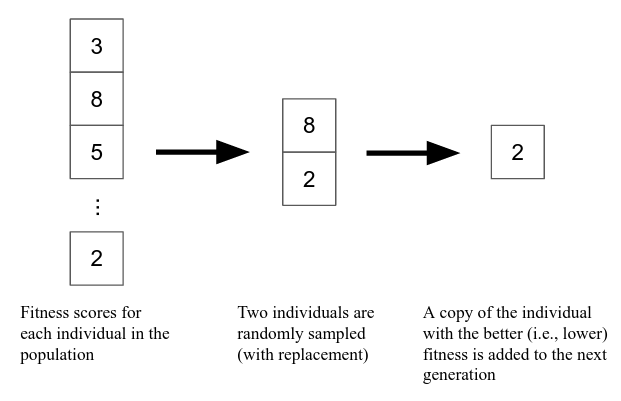
\includegraphics[width=8cm]{img/tournament.png}
\caption{An overview of the simple variant of tournament selection used in this work.
  Two mutants are randomly chosen and the winner with better fitness is selected.}
\label{fig:tourn}
\end{figure}
\fi

The default in this work is to represent mutants as ZX-diagrams and to use rewrite rules as mutation operators.
As is common in practical applications of genetic algorithms, we do not use any crossover operators though this is an attractive area for future exploration given the graphical nature of ZX-diagrams. % FIXME: cite
Lastly, we use \emph{tournament selection} to determine the surviving mutants at each generation.
In this selection method, $k_{tourn}$ mutants are selected to compete in a ``tournament'' from which a winner is chosen based on fitness.
This is repeated $n_{mutants}$ times with replacement to obtain a surviving population.
We use a simple variant of tournament selection in which $k_{tourn} = 2$ and the winner is simply the mutant with better (i.e., lower) fitness.


\subsection{Objective Functions}\label{sec:obj-funcs}

% look up ion trap papers, single qubit gates with 99.9 fidelity and two qubit with 99 fidelity. 10 perc difference in fidelity. chris ballance

Both the energy function (used in SA) and the fitness function (used in GA) are instances of an \emph{objective function}.
An objective function measures the ``goodness'' of a particular solution to an optimization problem.
For our purposes, we require an objective function that, given a ZX-diagram, provides a reasonable measure of the complexity of the circuit obtained via extraction.
For consistency, all objective functions are defined in such a way that a low score is better (i.e., a low score indicates low complexity).

The most straightforward objective function involves extracting a circuit and measuring its complexity directly.
A quantitative measure of circuit complexit is also useful for evaluating our optimization techniques.
Given a circuit $C$ in terms of single- and 2-qubit gates, we define its complexity $Comp(C)$ to be a weighted average of its single-qubit and 2-qubit gate counts:
\begin{align*}
  Comp(C) = 10 * (\text{\# 2-qubit gates}) + 1 * (\text{\# single-qubit gates})
\end{align*}
A scaling factor of 10 is chosen because 2-qubit gates are typically an order of magnitude more costly to implement than a single-qubit gate~\cite{campbell2017roads, ballance2016high}.
Note that \codeword{basic_optimization} is always applied to the extracted circuit.

% There are two possible high-level approaches to scoring: (1) extract the circuit and measure its complexity directly, or (2) measure some property of the ZX-diagram that is a reasonable proxy for the complexity of the associated circuit.
% Even if (1) is not used to guide search, we still require a quantitative measure of circuit complexity to analyze both our optimization methods and the estimates provided by some instance of (2).

However, extracting a circuit from the ZX-diagram every time we want to measure its complexity is costly.
For example, evolving a population of 50 mutants for 100 generations would require 5000 extractions.
Instead, we could measure some property of the ZX-diagram that is a reasonable proxy for $Comp(C)$ (where $C$ is the circuit obtained via extraction).
The following are candidate properties to serve as such a proxy:
% Instead, the following are several quantities of a ZX-diagram that may serve as reliable proxies for $Comp(C)$ (where $C$ is the circuit obtained via extraction):
\begin{itemize}
\item
  The number of edges
\item
  The density of the underlying graph
\item
  The centrality of the underlying graph
\end{itemize}
The ZX-diagram is assumed to be graph-like.

Measuring the ZX-diagram is clearly preferable but relies on the existence of a property that is sufficiently correlated to $Comp$.
Note that none of the above objective functions, including $Comp$, are normalized and therefore scores can only be compared between isomorphic ZX-diagrams.

\section{Circuit Optimization Strategies}

Here we describe how we use these congruences and search procedures for quantum circuit optimization.
We first outline our primary method which involves first applying off-the-shelf methods to obtain a simplified ZX-diagram and subsequently searching the space of equivalent ZX-diagrams generated by Equations \ref{eq:gen-io-lc} and \ref{eq:gen-io-pivot}.
We then describe an alternative, more general approach in which Equations \ref{eq:gen-io-lc} and \ref{eq:gen-io-pivot} are combined with simplification rules to form a single action set over which search is applied.


\begin{figure}[t]
\centering
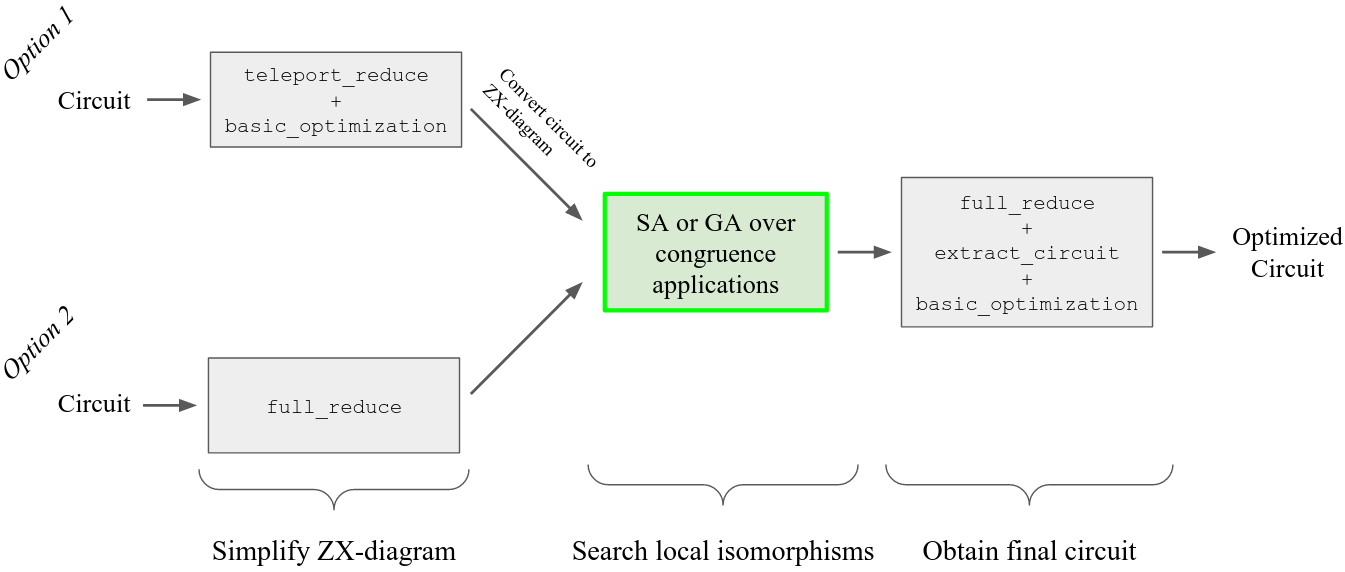
\includegraphics[width=15cm]{img/primary-overview.png}
\caption{
  An overview of our primary optimization strategy.
  Given an input circuit, a simplified ZX-diagram is obtained via one of two off-the-shelf methods.
  Then, we search for an equivalent ZX-diagram with similar graph complexity but lower circuit complexity (highlighted in green).
  A circuit is extracted from the final ZX-diagram and standard circuit-level optimizations are performed.
}
\label{fig:primary}
\end{figure}

\subsection{Primary: Post-Simplification Search}\label{sec:primary}

% changed from "the TR and FR pipelines described in Section ..."
Our primary optimization strategy improves upon the two pipelines described in Section \ref{sec:zx-circ-opt} by searching local variants of the simplified ZX-diagrams.
Given an input circuit, we can obtain a simplified ZX-diagram to seed search in one of two ways.
Firstly, we can apply \codeword{full_reduce}.
Importantly, we do not apply the entire \codeword{full_reduce} + \codeword{extract_circuit} + \codeword{basic_optimization} pipeline and convert the simplified circuit to a ZX-diagram as the complexity cost incurred by extraction will likely outweigh any simplifications achieved at the circuit-level.
Alternatively, since \codeword{teleport_reduce} short-circuits circuit extraction, we can apply \codeword{teleport_reduce} + \codeword{basic_optimization} and convert the simplified circuit to a ZX-diagram.
Given a simplified ZX-diagram, we can then apply SA or GA to search the space of ZX-diagrams generated by Equations \ref{eq:gen-io-lc} and \ref{eq:gen-io-pivot} for an equivalent ZX-diagram whose extracted circuit is less complex.
Note that search proceeds by first randomly selecting one of Equations \ref{eq:gen-io-lc} and \ref{eq:gen-io-pivot} and then randomly selecting a subject (i.e., spider or pair of connected spiders) for the selected congruence.
We denote the probability of selecting Equations \ref{eq:gen-io-lc} and \ref{eq:gen-io-pivot} as $p_{LC}$ and $p_{pivot}$, respectively (default: $p_{LC} = p_{pivot} = 0.5$).
An overview of this strategy is depicted in Figure \ref{fig:primary}.
% Note: Could alternatively have the "cloud" figure with graph complexity vs circuit complexity.

Since Equations \ref{eq:gen-io-lc} and \ref{eq:gen-io-pivot} break the circuit structure of a graph, it is reasonable to apply \codeword{full_reduce} because a circuit has to be extracted regardless.
Therefore, the default objective function scores a ZX-diagram by first applying \codeword{full_reduce}, extracting a circuit $C$ and applying simple circuit-level optimizations with \codeword{basic_optimization}, and measuring its complexity $Comp(C)$.
We can also apply \codeword{full_reduce} probabilistically via some free parameter $p_{fr}$ throughout search (default: $p_{fr} = 0.1$).
In SA, \codeword{full_reduce} is applied to the current state at each step with probability $p_{fr}$ while in GA \codeword{full_reduce} is applied to each mutant in a given generation with probability $p_{fr}$.

There are several opportunities to refine this strategy.
One example is applying Equations \ref{eq:gen-io-lc} and \ref{eq:gen-io-pivot} with unequal probabilities.
This could be beneficial if one congruence more effectively navigates the search space than the other.
Another possible refinement is non-uniform sampling of spiders (resp. pairs of spiders) to which Equation \ref{eq:gen-io-lc} (resp. Equation \ref{eq:gen-io-pivot}) will be applied.
The following are possible spider metrics to weight sampling for application of Equation \ref{eq:gen-io-lc}:
\begin{itemize}
\item
  Degree
\item
  Centrality (e.g., betweenness, Katz)
\item
  Total degree of neighbors
\end{itemize}
Similarly, the following are possible metrics to weight sampling of pairs of nodes for Equation \ref{eq:gen-io-pivot}:
\begin{itemize}
\item
  Sum of spider-wise metrics (e.g., total degree of the union of all neighbors)
\item
  Edge centrality (e.g., load, betweenness)
\item
  Edge dispersion
\end{itemize}
Lastly, we can experiment with different values of $p_{fr}$.


\subsection{Alternative: Congruences as First-Class Citizens}

An underlying assumption of \codeword{full_reduce} is that simplifying the ZX-diagram as much as possible is optimal.
However, removing spiders to fixpoint may come at a cost.
For example, later-stage spider removals may induce connectivity properties in the ZX-diagram (e.g., high-degree spiders, high density) that translate to a high 2-qubit count upon extraction.

To test this, we employ an alternative simplification strategy in which congruences are applied alongside simplifications rather than after the ZX-diagram is fully simplified.
More specifically, we treat individual simplification rules as actions and combine these with Equations \ref{eq:gen-io-lc} and \ref{eq:gen-io-pivot} to form a master action set.
These individual simplifications are the following: \textcolor{red}{FIXME itemize, and then a sentence on what they can be applied to}.
Given an input circuit, we convert it to a ZX-diagram and search over this master action set.
For search, we only use GA as maintaining a population of mutants rather than a single state (as in SA) is well-suited for the significantly higher branching factor.

\textcolor{red}{FIXME: If have time and space, can extend to the case where the state of GA is both circuit + ZX-diagram so that we can apply non-PyZX simplifications.}

% because going to fixpoint might be bad. go global instead. use all. congruences as first-class citizens
% Only use GA for this because handles branching factor better. can repr states as pairs so we can do non-pyzx optimizations! mutation operators take in pair and return apir. in practice, this owrks in one of two ways.





% only use GA as branching factor is too big

% Maybe simplifying to fixpoint isn't optimal, and introduces too many edges that lead to CNOTs to get us marginal T-count gain. So, we can just be careful right from the beginning!

% subsection: from scratch. just include congruences as a possible action along with all the others
% In this work, mutants are represented as pairs of ZX-diagrams and their associated circuits by default.
% This allows for mutation to occur at either the graph- or circuit-level.
% If a mutant is modified at the graph-level (i.e., via a rewrite rule), the associated circuit is obtained via extraction.
% Alternatively, traditional circuit-level optimizations can be applied and the correpsonding ZX-diagram can be generated directly from the modified circuit..
% mutation operator takes in a pair and returns a pair.

% (archived) -- FIXME: Other, more general combinations (e.g., GA with all simps, or search with other ``safe'' procedures).

\chapter[Results]{Results} \label{ch:results}

% Here we present the results of our primary and alternative optimization strategies.
Here we present the results of our optimization strategy.
Before reporting on the performance of our strategy, we first conduct preliminary analyses to refine our method.
% After finalizing these refinements, we report on the performance of this strategy.
All random circuits are generated using the \codeword{CNOT_HAD_PHASE_circuit} method in PyZX which constructs a circuit consisting of CNOT, HAD, and phase gates.
Default parameters are used for the probability of each gate type.


% \section{Primary Strategy}

\section{Refinements}

General opportunities for refinement are the following:
\begin{itemize}
\item
  Optimization function
\item
  Probability of applying Equation \ref{eq:gen-io-lc} vs. Equation \ref{eq:gen-io-pivot}
\item
  Sampling of subjects (i.e., spiders or pairs of connected spiders) for congruence application
% \item
  % Probability of applying \codeword{full_reduce} throughout search, $p_{fr}$ % FIXME: Could just skip this one...
\end{itemize}
For these analyses, we only use SA as it is more computationally efficient and we expect the behavior of these refinements to generalize to GA.

We also conduct procedure-specific refinements.
We analyze how varying the number of iterations or mutants and generations affects optimization using SA and GA, respectively.

\subsection*{Optimization Function}

First, we test if any property of a ZX-diagram could serve as a reliable proxy for the complexity of its associated circuit.
To do so, we first generated 500 random circuits (10 qubits, 100 gates) and immediately converted them to ZX-diagrams.
Given this library of ZX-diagrams, we then measured the Pearson correlation coefficient between the complexity of the extracted circuit and each ZX-diagrammatic property discussed in Section \ref{sec:obj-funcs}.
The following table summarizes these correlations:
\begin{center}
  % \begin{table*}[h!]
  % \begin{tabular}[]{@{}lcc@{}}
\begin{tabular}[]{@{}l>{\centering\arraybackslash}p{1.5cm}>{\centering\arraybackslash}p{2cm}@{}}
\toprule
                    & $r$ & p-value \\ \midrule
\# Edges  & 0.097        & 0.029            \\
Centrality & 0.090        & 0.045            \\
Density    & -0.096       & 0.032            \\ \bottomrule
\end{tabular}
% \caption{\label{tab:obj-pearson}Correlations between various ZX-diagrammatic properties and the complexity of the extracted circuit for 500 randomly generated ZX-diagrams. Pearson's correlation coefficient is denoted $r$ and the 2-tailed p-value is provided. The ZX-diagrams were generated by converting 500 random circuits with 10 qubits and 100 gates to ZX-diagrams.}
% Table \ref{tab:obj-pearson} summarizes these correlations.
% \end{table*}
\end{center}
Pearson's correlation coefficient is denoted $r$ and the 2-tailed p-value is provided.
From these data, it is clear that no identified property of a ZX-diagram can serve as a reliable proxy for the complexity of its associated circuit.
Therefore, the default scoring method discussed in Section \ref{sec:strategy} that relies on extraction is used for the remainder of our analyses.



\begin{figure}[t]
\centering
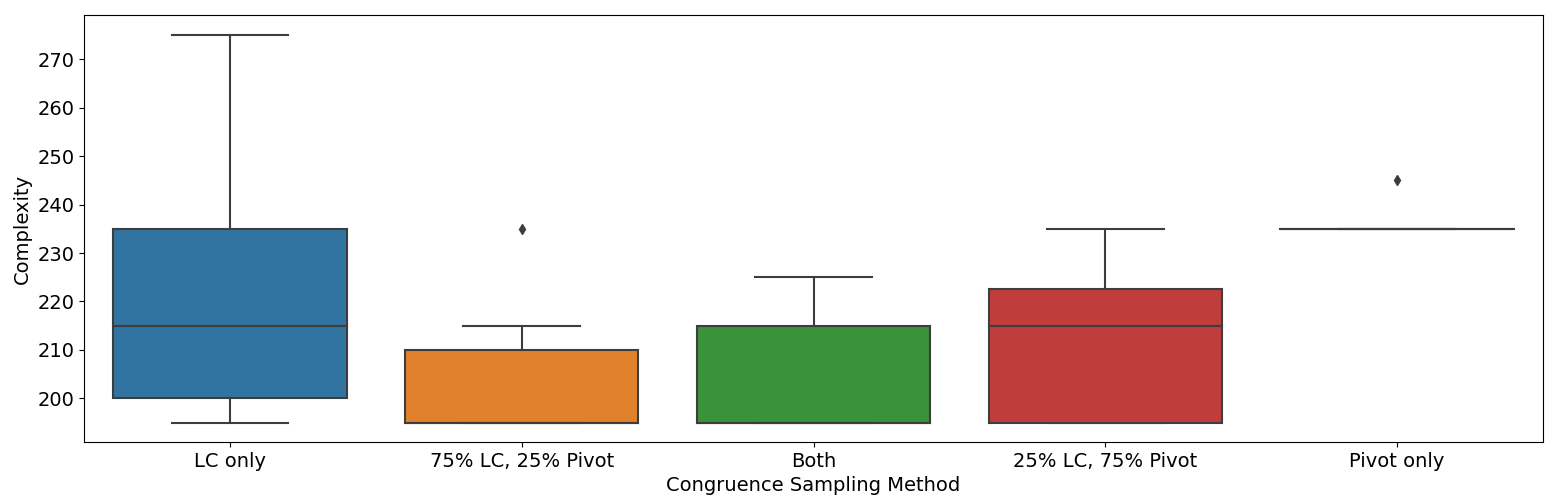
\includegraphics[width=13cm]{img/cong-sampling-ex.png}
\caption{
  A representative comparison of congruence sampling methods for a 5 qubit, 50 gate circuit.
  All three sampling methods that include both LC and pivoting achieve the best simplification in the alotted number of steps.
  When using only local complementation (i.e., Equation \ref{eq:gen-io-lc}), the same best-case complexity is achieved over the 10 trials but the average complexity is higher.
  Alternatively, using only pivoting does not achieve the same reduced circuit.
}
\label{fig:cong-sampling}
\end{figure}

\subsection*{Congruence Sampling}

By default, we apply Equations \ref{eq:gen-io-lc} and \ref{eq:gen-io-pivot} with equal probability ($p_{LC} = p_{pivot} = 0.5$).
However, it may be the case that one congruence should be chosen more frequently than the other.
To evaluate this, we generated 30 random circuits (5 qubits, 50 gates) and repeated search with a range of $(p_{LC}, p_{pivot})$ pairs.
For a given circuit, search was performed 10 times for each pair and the complexities of the optimized circuits were plotted according to congruence sampling probabilities.
In all cases, the sampling methods that include both LC and pivoting yielded the lowest average complexity across the 10 trials as well as the least complex circuit overall.
% In some cases, other sampling methods matched, but never outperformed this method in either metric.
There were no significant differences between the three combined sampling methods (i.e., 50/50, 25/75, and 75/25) and the LC- ($p_{LC} = 1.0$, $p_{pivot} = 0.0$) or pivot-only ($p_{LC} = 0.0$, $p_{pivot} = 1.0$) sampling methods sometimes matched, but never outperformed these combined methods.
% Most notably, the least cusing only local complementation (i.e., $p_{LC} = 1.0$, $p_{pivot} = 0.0$) produced a circuit that matched the
Most notably, the least complex circuit identified using LC-only matched the minimum complexity 73.3\% of the time while that identified using pivot-only was more complex than the best-case 86.7\% of the time.
% Most notably, the least complex circuit identified using only local complementation (i.e., $p_{LC} = 1.0$, $p_{pivot} = 0.0$) matched the minimum complexity found via 50/50 sampling FIXME\% of the time and was less complex than that found using only pivoting FIXME\% of the time (and otherwise no more complex).
% Most notably, the minimum-complexity circuit identified using LC-only (i.e., $p_{LC} = 1.0$, $p_{pivot} = 0.0$) matched that found via 50/50 sampling
% method most commonly matched the default and almost always outperformed the pivot-only method.
% LC-only (i.e., $p_{LC} = 1.0$, $p_{pivot} = 0.0$) and
A representative comparison for one random circuit is shown in Figure \ref{fig:cong-sampling}.

The observation that LC-only typically outperforms pivot-only is intuitive as one pivot is equivalent to three local complementations and therefore LC-only enables a more fine-grained search.
While LC-only likely converges to the combined sampling methods in the limit, we retain pivoting in the action set as it appears to require a fewer number of iterations at no cost.
% However, since LC-only always matches and never outperforms the equal sampling of either congruences,
In the remainder of our analyses, the default uniform sampling of Equations \ref{eq:gen-io-lc} and \ref{eq:gen-io-pivot} (i.e., $p_{LC} = p_{pivot} = 0.5$) is used.


\begin{figure}[t]
\centering
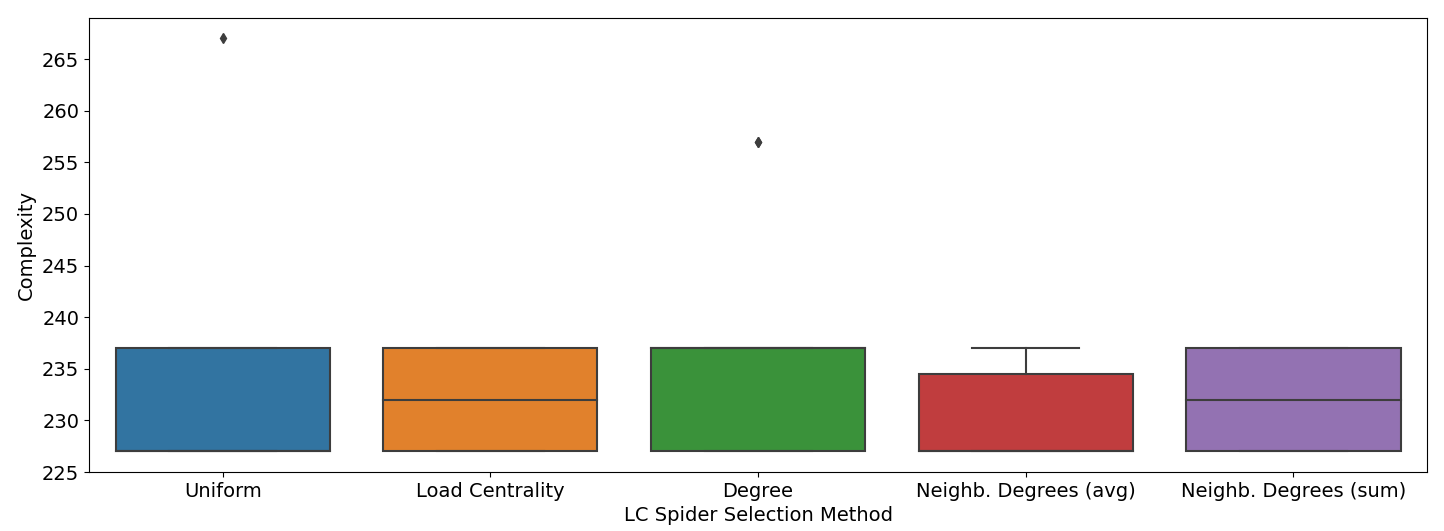
\includegraphics[width=13cm]{img/subj-sampling-ex.png}
\caption{
  A representative example of optimization of a 5 qubit, 50 gate circuit with different metrics of sampling spiders for application of Equation \ref{eq:gen-io-lc}.
  Optimization was performed 10 times for each sampling method using SA.
  No significant differences are observed in performance across the different weightings.
}
\label{fig:subj-sampling}
\end{figure}


\subsection*{Congruence Subject Sampling}

Similar to the probabilistic sampling of congruences to apply throughout search, we can experiment with methods of sampling subjects (i.e., spiders or pairs of connected spiders) for congruence application.
By default, we sample from the set of all eligible subjects uniformly.
However, we could alternatively weight this sampling in a way that improves search.
Candidate metrics for Equations \ref{eq:gen-io-lc} and \ref{eq:gen-io-pivot} are discussed in Section \ref{sec:strategy}.

To test these alternative weightings, we employ a similar approach as for congruence sampling.
First, we restrict the action space to that congruence for which we are testing various weightings to isolate its effect.
For example, if we are testing various weighting metrics to select a spider for application of Equation \ref{eq:gen-io-lc}, we set $p_{LC} = 1.0$ and $p_{pivot} = 0.0$.
We then proceed as before, evaluating the performance of SA on random circuits across 10 trials for each candidate weighting.
We evaluate 20 random circuits (5 qubits, 50 gates) for each set of sampling procedures.

In both cases, no sampling method demonstrated reliable improvement over any other across the 20 trials.
One representative example of this comparison for sampling spiders for Equation \ref{eq:gen-io-lc} is shown in Figure \ref{fig:subj-sampling}.
Similar results were observed for sampling pairs of connected spiders for Equation \ref{eq:gen-io-pivot}.
So, for the remainder of our analyses, we sample subjects for congruence application uniformly.

\begin{figure}[t]
\centering
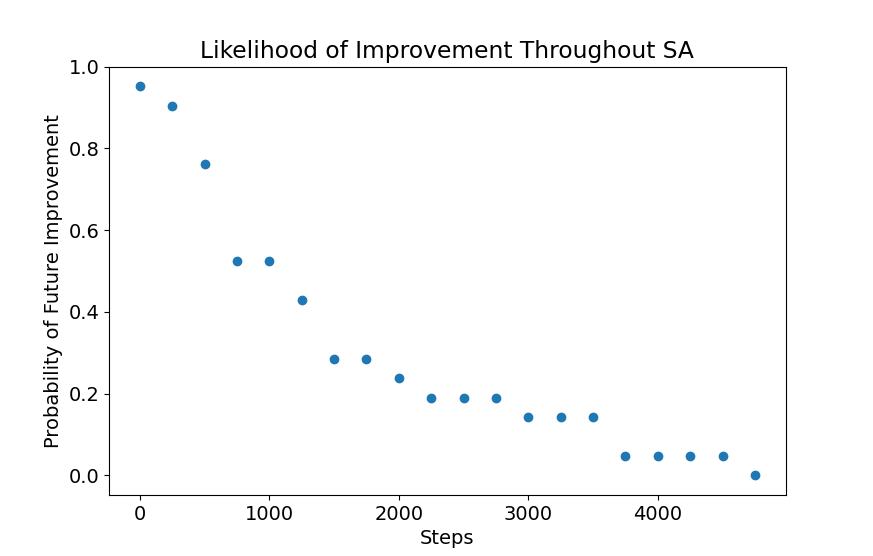
\includegraphics[width=13cm]{img/iter-likelihood.png}
\caption{
  The likelihood of obtaining a ZX-diagram with a simpler extracted circuit after a given iteration in SA.
  For example, after 2000 steps, there is a 20\% chance of obtaining a ZX-diagram corresponding to an even simpler circuit as search progresses.
  These data were obtained using circuits with 4-10 qubits and 10-20 gates per qubit and do not necessarily generalize to larger circuits.
}
\label{fig:iter-likelihood}
\end{figure}

\subsection*{Number of SA Iterations}

The maximum number of SA steps $k_{max}$ should be high enough to permit the bulk of optimization while low enough to be computational feasible.
We determine the optimal $k_{max}$ by optimizing a set of random circuits and computing the probability that SA uncovers a complexity reduction after fixed intervals.
First, we generated a set of 36 random circuits with 4-10 qubits (intervals of 2) and 10-20 gates per qubit (intervals of 5).
For each circuit, we obtained a simplified ZX-diagram via \codeword{teleport_reduce} + \codeword{basic_optimization}.
We then optimized each simplified ZX-diagram using SA with $k_{max} = 5000$ and recorded the complexity of the best circuit every 250 steps.
Lastly, we computed the probability that a ZX-diagram whose extracted circuit is less complex would be found as search progressed for each 250-step interval.
% Lastly, we computed the probability that a less-complex circuit would be found as search progressed for each 250-step interval.
% We repeated this entire analysis twice, once for each method of obtaining a simplified ZX-diagram from a circuit (see Figure \ref{fig:primary}).

The results of this analysis are shown in Figure \ref{fig:iter-likelihood}.
We see that most improvement occurs in the beginning of search and that the chance of finding a simpler circuit after 2500 steps is less than 10\%.
For this reason, we fix $k_{max} = 2500$ for the remainder of our analyses unless otherwise noted.


\begin{figure}
\centering
\begin{subfigure}[t]{0.47\textwidth}
  \centering
  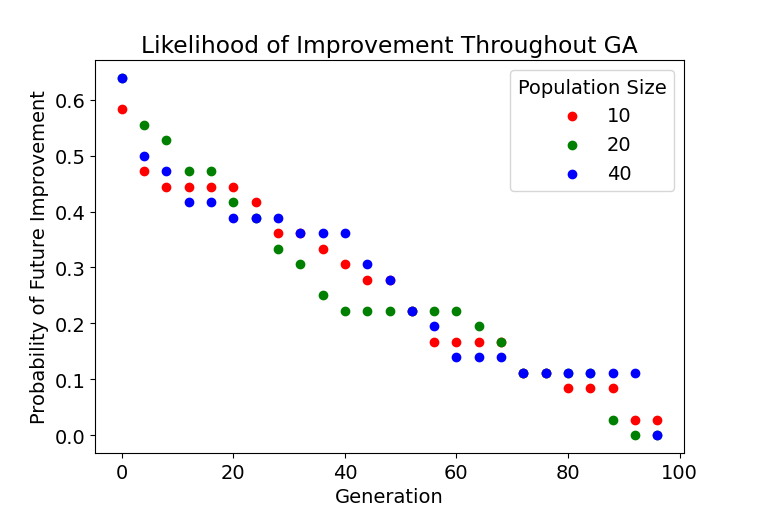
\includegraphics[width=\linewidth]{img/ga-likelihood.png}
  \caption{The likelihood of obtaining a simpler circuit after a given generation.
  As in Figure \ref{fig:iter-likelihood}, these data were obtained using circuits with 4-10 qubits and 10-20 gates per qubit.}
  \label{fig:ga-likelihood}
\end{subfigure}
\hfill
\begin{subfigure}[t]{0.47\textwidth}
  \centering
  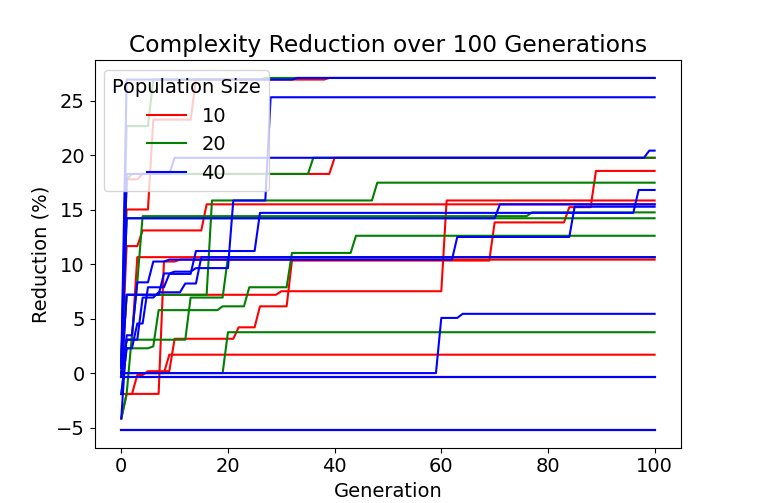
\includegraphics[width=\linewidth]{img/7qb}
  \caption{
    The reduction in complexities over time for 10 random 7 qubit, 100 gate circuits.
    Reduction in complexity is measured with respect to the simplified ZX-diagram rather than the original circuit.
  }
  \label{fig:7qb}
\end{subfigure}
\caption{
  GA parameter tuning
}
\label{fig:ga-params}
\end{figure}


\iffalse
\begin{figure}[t]
\centering
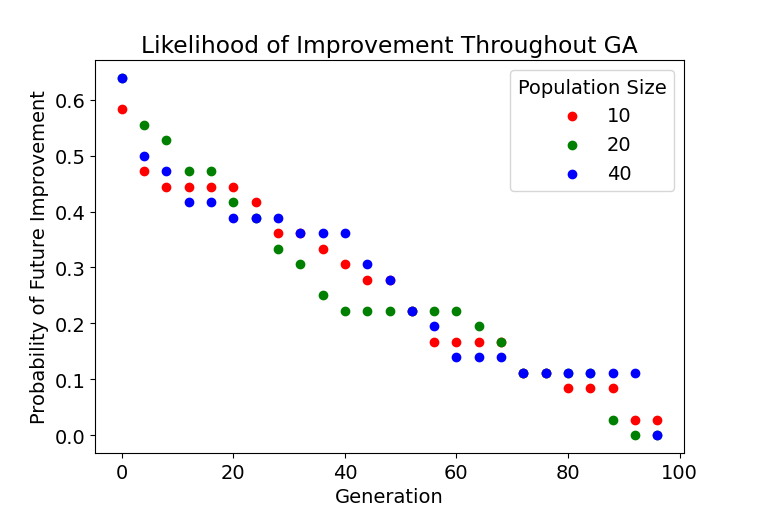
\includegraphics[width=13cm]{img/ga-likelihood.png}
\caption{
  The likelihood of obtaining a ZX-diagram corresponding to a simpler circuit after a given generation in GA.
  As in Figure \ref{fig:iter-likelihood}, these data were obtained using circuits with 4-10 qubits and 10-20 gates per qubit.
}
\label{fig:ga-likelihood}
\end{figure}
\fi


\subsection*{GA Parameters}

Similarly, when searching this space with GA, we want to evolve a large enough population for sufficiently many generations while incurring minimal computational cost.
To determine the appropriate population size and number of generations, we employ a similar approach as for determining $k_{max}$.
First, we generated a set of 36 simplified ZX-diagrams in the same fashion.
We then evolved each ZX-diagram for 100 generations with a population of 10, 20, or 40 mutants.
Lastly, for each population size, we computed the probability that a ZX-diagram corresponding to a simpler circuit (via extraction) would be found as search progressed for each 2-generation interval.
These probabilities for each population size are shown in Figure \ref{fig:ga-likelihood}.
Interestingly, all three population sizes exhibit similar behavior.
% Additionally, almost 50\% of all evolutions either perform all optimization in the 0th generation or provide no improvement.

We also sought to understand both the rate of reduction (with respect to the simplified ZX-diagram) over time and differences in total reduction between population sizes.
We plotted the complexity reduction over time for 10 random circuits with 7 qubits and 100 gates for each population size.
% We also generated 10 random circuits with 7 qubits and 100 gates and plotted the complexity reduction
% We also plot the complexity reduction (with respect to the simplified ZX-diagram) over time for each circuit both to evaluate the rate of reduction and to identify differences in total reduction between population sizes.
These reductions (one line per circuit for each population size) are shown in Figure \ref{fig:7qb}.
% note that there is particularly high variance in performance as the circuits have a variable number of qubits.
It is immediately clear that most optimization occurs in the first few generations.
Additionally, there is no reliable benefit provided by a larger population size.
We fix $n_{mutants} = 20$ and $n_{gens} = 40$ for the remainder of our analyses unless otherwise stated.

\section{Performance}

After refining the parameters of our method, we seek to understand our method's overall capabilities.

\subsection*{Further Simplification of ZX-Diagrams}

First, we want to understand our procedure's ability to further optimize a simplified ZX-diagram.
In this sense, we are not (yet) comparing the two methods of obtaining this initial ZX-diagram and complexity reduction is measured with respect to the simplified ZX-diagram that seeds search.
We test this by optimizing the simplified ZX-diagrams of 10 randomly generated circuits for $4, 6, \dots 14$ qubits with either 10 or 25 gates per qubit.
% First: Reduction capabilities for either TR or FR input. Not comparing TR vs. FR. Show for both SA and GA. This is telling us performance with respect to qubits, and also SA vs GA.
% First, we test the performance of our procedure for varying circuit sizes.
% Given a simplified ZX-diagram, we are initially only interested in our procedure's ability to further optimize the corresponding circuit;
% % Importantly, we are initially only interested in the reduction in complexity from the circuit associated with the simplified ZX-diagram rather than the original circuit.
% in this sense, we are not (yet) comparing the two methods of obtaining this initial ZX-diagram.
% For $4, 6, \dots 14$ qubits, we optimize the simplified ZX-diagrams of 10 randomly generated circuits with either 10 or 25 gates per qubit.
% We then plot the average reduction with respect to the simplified ZX-diagram.
We repeat this analysis for all four combinations of the two search procedures and the two ZX-diagram simplification methods.

Figure FIXME contains plots of average reductions for all four combinations.
% FIXME: analysis. most likely can always provide benefit, and SA and GA are similar. cant for higher qubits, and might make more progress on the FR one.


% \subsection*{Comparison of Search Procedures and Initial Simplifications}
\subsection*{Improving Optimization of the Original Circuit}

% Okay, we know we can improve on the simplified ZX-diagram. Now, want to compare for performance on input circuit.
After demonstrating that our method can further simplify ZX-diagrams for circuits with a sufficiently low number of qubits, we want to understand how these graph-level simplifications translate to optimization of the original circuit.

% Then, if we are concerned with optimizing the input circuit, is it better to apply congruences over FR or TR + basic simplified ZX-diagram? Compute some averages, and show a representative histogram with vertical lines.

% Then, took benchmarks from previous paper below qubit threshold. Did better.

\subsection*{Scaling Efforts}

% Then, we see if we can get higher qubits. Increase iterations, etc.

Lorem ipsum. I said lorem ipsum.

\begin{table}[]
\begin{tabular}{@{}ccccccc@{}}
\toprule
\multirow{3}{*}{\textbf{Qubits}}           & \multicolumn{6}{c}{\textbf{Complexity Reduction (\%)}}                                                      \\ \cmidrule(l){2-7}
                                           & \multirow{2}{*}{TR} & \multirow{2}{*}{FR} & \multicolumn{2}{c}{SA} & \multicolumn{2}{c}{GA} \\ \cmidrule(l){4-7}
                                           &                     &                     & TR seed    & FR seed   & TR seed    & FR seed   \\ \midrule
4                                          & 10                  & 10                  & 10         & 10        & 10         & 10        \\
6                                          & 10                  & 10                  & 10         & 10        & 10         & 10        \\
8                                          & 10                  & 10                  & 10         & 10        & 10         & 10        \\
10                                         & 10                  & 10                  & 10         & 10        & 10         & 10        \\
12                                         & 10                  & 10                  & 10         & 10        & 10         & 10        \\
14                                         & 10                  & 10                  & 10         & 10        & 10         & 10        \\ \midrule
\multicolumn{1}{l}{\textbf{Avg. Time (s)}} & 1                   & 1                   & 100        & 100       & 100        & 100       \\ \bottomrule
\end{tabular}
\end{table}

\chapter[Discussion and Conclusion]{Discussion and Conclusion} \label{ch:discuss-conc}

Lorem ipsum dolor sit amet, consectetur adipiscing elit, sed do eiusmod tempor incididunt ut labore et dolore magna aliqua. Ut enim ad minim veniam, quis nostrud exercitation ullamco laboris nisi ut aliquip ex ea commodo consequat.

% extraction is bottleneck
% time isn't really an issue
% search space doesn't seem to be that broad. quick to local minima


%now enable appendix numbering format and include any appendice
% \appendix
% \chapter[Proofs]{Proofs} \label{ch:a1}

\kant[1-3]
{\allowdisplaybreaks
\begin{align*}
left &= right1 \\
     &= right2.
\end{align*}}
Here we include the proof for generalized local complementation:
{\allowdisplaybreaks
\begin{align*}
  \tikzfig{gen-lc-proof/0} &= \tikzfig{gen-lc-proof/1} \\
  &= \tikzfig{gen-lc-proof/2} \\
  &= \tikzfig{gen-lc-proof/3} \\
  &= \tikzfig{gen-lc-proof/4} \\
  &= \tikzfig{gen-lc-proof/5}
\end{align*}}
% \ctikzfig{gen-lc-full}

% \include{appendix2}

%next line adds the Bibliography to the contents page
\addcontentsline{toc}{chapter}{Bibliography}
%uncomment next line to change bibliography name to references
%\renewcommand{\bibname}{References}
\bibliography{refs}        %use a bibtex bibliography file refs.bib
\bibliographystyle{plain}  %use the plain bibliography style

\end{document}
